\chapter{Introduction}

Explain the context of your essay topic, so that the
topic itself appears motivated, natural and important.

\begin{figure}[h]
\psfrag{A}{$d^2$}
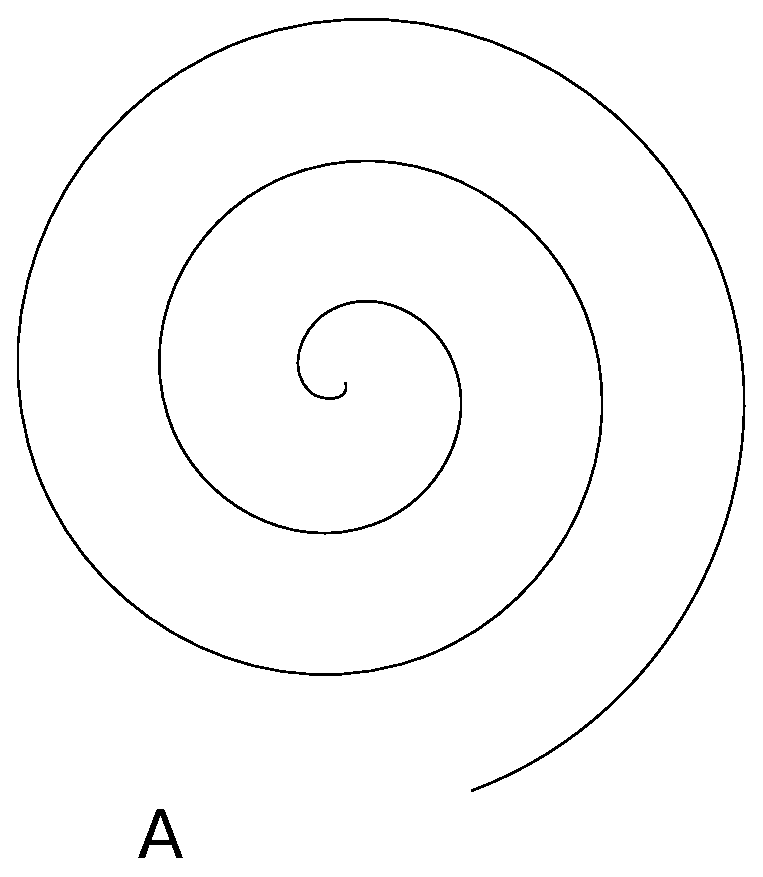
\includegraphics[scale=0.5]{images/drawing.eps}
\end{figure}

Paragraphs are separated by blank lines in the \LaTeX\ code, 
and the line spacing, paragraph indentation,
and paragraph spacing are set in the preamble for you, 
according to AIMS house style.

This is a textual citation \citet{shannon44}. And this is a parenthetical citation \citep{shannon44}. You probably want to use the latter more often.

\section{Moving On}
Let's demonstrate a figure by looking at Fig.~\ref{bandwidth}. 

\begin{figure}[!h]
% Use "\centering" in floats (figure, table), but if you need to center
% some text (why?) use "\begin{center}...\end{center}".
\centering 
% Figure environments same as 0.8 * \textwidth please
% That does not necessarily mean the actual picture size,
% it is a guideline for the environment which could contain
% 2 or more pictures! Be consistent and follow the guidelines
% provided in your sources.
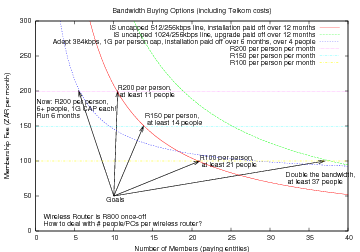
\includegraphics[width=0.8\textwidth]{images/bandwidth-colour.png}
\caption{Planning community bandwidth sharing costs. 
  Note caption capitalization.}
\label{bandwidth} 
% if you move the label it breaks the reference numbering; 
% always have it *after* the caption.
\end{figure}

Remember how to include code with {\tt verbatim} 
and to fix the tabs in {\sf python} in a verbatim environment? 
It may be best to have an `include' command for code, 
not to have to re-edit it all the time.
\verbatimtabinput{code/mycode.py}


